\documentclass[t]{beamer}
\usepackage{default}
\usepackage[]{graphicx}
\usepackage{amsfonts}
\usepackage{amssymb}
\usepackage{amsmath}
\usepackage[brazil]{babel}
\usepackage[utf8]{inputenc}
\usepackage[T1]{fontenc}
\usepackage{lmodern}
\usepackage{hyperref}
\usepackage{listings}
\usetheme{Dresden}

\author{Thiago de Gouveia Nunes}
\title{Registro de Imagens\\ Demons versus TPS}
\institute{IME - USP}

\setbeamertemplate{navigation symbols}{}
\setbeamertemplate{bibliography item}{}
\setbeamertemplate{frametitle continuation}[from second]

\newcommand{\frameofframes}{/}
\newcommand{\setframeofframes}[1]{\renewcommand{\frameofframes}{#1}}

\setframeofframes{/}
\makeatletter
\setbeamertemplate{footline}
  {%
    \begin{beamercolorbox}[colsep=1.5pt]{upper separation line foot}
    \end{beamercolorbox}
    \begin{beamercolorbox}[ht=2.5ex,dp=1.125ex,%
      leftskip=.3cm,rightskip=.3cm plus1fil]{author in head/foot}%
      \leavevmode{\usebeamerfont{author in head/foot}\insertshortauthor}%
      \hfill%
      {\usebeamerfont{institute in head/foot}\usebeamercolor[fg]{institute in head/foot}\insertshortinstitute}%
    \end{beamercolorbox}%
    \begin{beamercolorbox}[ht=2.5ex,dp=1.125ex,%
      leftskip=.3cm,rightskip=.3cm plus1fil]{title in head/foot}%
      {\usebeamerfont{title in head/foot}\insertshorttitle}%
      \hfill%
      {\usebeamerfont{frame number}\usebeamercolor[fg]{frame number}\insertframenumber~\frameofframes~\inserttotalframenumber}
    \end{beamercolorbox}%
    \begin{beamercolorbox}[colsep=1.5pt]{lower separation line foot}
    \end{beamercolorbox}
  }
\makeatother

\begin{document}
\graphicspath{{images/}}
\frame{\titlepage}

\section{Revisão de Registro}
\subsection{}

\begin{frame}
    O registro de imagens tem como objetivo alinhar duas imagens diferentes. \\
    Dentro de processamento de imagens médicas o registro é usado como uma ferramenta auxiliar em vários estudos, entre eles:
    \begin{itemize}
        \item Retirar deformações resultantes da movimentação do paciente ou do seus tecidos;
        \item Retirar características individuais em estudos populacionais.
    \end{itemize}
    O registro pode ser classificado quanto ao tipo de deformação que ele tenta restaurar:
    \begin{itemize}
        \item Transformações afins, ou lineares;
        \item Transformações não afim, ou não lineares.
    \end{itemize}
\end{frame}

\begin{frame}
    O algoritmo de registro recebe como entrada duas imagens, a imagem de referência (R) e a alvo (A). \\
    Cada algoritmo utiliza um método diferente para calcular um campo vetorial que é aplicado a imagem alvo a fim de alinhá-la
com a imagem referência.

\end{frame}

\begin{frame}
   \begin{columns}[c]
      \column{.5\textwidth}
        \begin{figure}[!h]
          \begin{center}
            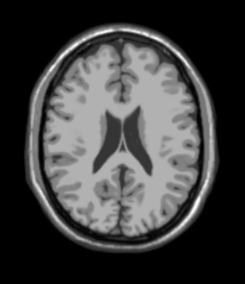
\includegraphics[width=1.0\textwidth]{../images/screen.png}
            \caption{Imagem Referência.}
          \end{center}
        \end{figure}
      \column{.5\textwidth}
        \begin{figure}[!h]
          \begin{center}
            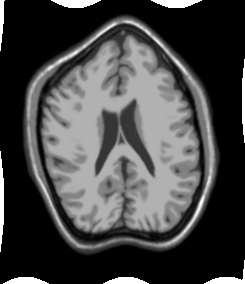
\includegraphics[width=1.0\textwidth]{../images/movingImageSin.png}
            \caption{Imagem Alvo.}
          \end{center}
        \end{figure}
    \end{columns}
\end{frame}

\begin{frame}
Esse trabalho tem como objetivo a comparação dos métodos \textit{Demons}\cite{thirion1995fast} e 
\textit{Thin Plate Splines}\cite{goshtasby1988registration} (TPS) para recuperar deformações aplicadas a imagens médicas.
Eles são algoritmos especializados em registro não linear.
\end{frame}

\section{Demons}
\subsection{}
\begin{frame}
O Demons tem como base o modelo de atratores, em que pontos são
definidos das duas imagens e os pontos da imagem alvo são atraídos por pontos da imagem referência usando alguma 
métrica.

O Demons aplica uma dimensão de informação a mais ao modelo de atratores, acrescentando a cada ponto uma direção
associada ao gradiente da imagem. Cada atrator no Demons é chamado de Demon.
\end{frame}

\begin{frame}
  O Demons supõe que a transformação só movimenta os pixeis e não muda suas intensidades.
  \begin{align}
    \begin{split}
    i(x(t),y(t),z(t)) = const \\
    \end{split}
  \end{align}
  Derivando (1) temos:
  \begin{align}
    \frac{\partial i}{\partial x} \frac{\partial x}{\partial t} +
    \frac{\partial i}{\partial y} \frac{\partial y}{\partial t} = - \frac{\partial i}{\partial t}
\end{align}
\end{frame}

\begin{frame}
        Supondo que as duas imagens que temos diferem de uma unidade de tempo $\partial i/\partial t = 
r-a$, \textit{r} e \textit{a} as intensidades de R e A respectivamente e que a velocidade instantânea 
$\vec{v} = (dx/dt,dy/dt)$ é aplicada a cada pixel para movê-lo de A para R, chegamos a equação:
\begin{align}
    \vec{v}*\vec{\nabla}r = a - r, \ \text{onde} \ \vec{\nabla} r \ \text{é o gradiente de R}
\end{align}
\end{frame}

\begin{frame}
    O Demons é um algoritmo iterativo. Como entrada ele recebe a imagem referência e alvo e possivelmente um campo
vetorial inicial. Seus passos são:
\begin{itemize}
    \item Para cada Demon em $A_i$, calculamos $\vec{v_i}$, criando um novo campo vetorial $V_i$
    \item Aplicamos um filtro Gaussiano para retirar o ruido introduzido pelo processo em $V_i$
    \item Aplicamos $V_i$ em $A$ para obter $A_{i+1}$;
\end{itemize}
\end{frame}

\begin{frame}
    No artigo que define o Demons, o autor também cria uma variação dele, chamada de Demons Simétrico. \\
O método simétrico utiliza o gradiente da imagem deformada para calcular a próxima iteração:
\begin{align}
    \vec{v} = \frac{4(a - r)*\vec{\nabla}r|\vec{\nabla}r||\vec{\nabla}a|}
                    {(\vec{\nabla}r+\vec{\nabla}a)^2*(\vec{\nabla}r^2 + \vec{\nabla}a^2 + 2(a - r)^2)}
\end{align} 
\end{frame}

\section{Thin-Plate Splines}
\subsection{}

\begin{frame}
    O Thin Plate Splines (TPS) utiliza um outro paradigma para realizar o registro de imagens. Ele utiliza
    características para criar uma função de interpolação que é utilizada para criar a imagem registrada a partir
    da imagem referência.

    Dados as características na imagem referência $(x_i,y_i, i=1,..,n)$ e na imagem alvo $(X_i,Y_i, i=1,..,n)$
o TPS cria uma função que mapeia exatamente cada característica da imagem referência na sua
correspondente na imagem alvo e que é capaz de interpolar os pontos restantes para a imagem final.
\end{frame}

\begin{frame}
Para realizar
essa tarefa é utilizada uma função que define uma superfície que sofre a ação de pesos centrados nas
características da imagem referência. A superfície é definida pela seguinte equação\cite{bookstein1989principal}:

\begin{align}
    f(x,y) = A_0 + A_1x + A_2y + \sum_{i=0}^n F_i r_i^2 ln r_i^2
\end{align}
Onde $r_i^2 = (x-x_i)^2 + (y-y_i)^2 + d^2$, $d$ é um fator de rigidez da superfície, quanto mais próximo de 
zero $d$ é mais a superfície sofre ação dos pontos de controle, e os pontos $(x_i, y_i)$ são os pontos de controle.
\end{frame}

\begin{frame}
    O TPS deve então determinar os valores das variáveis $A_0, A_1, A_2$ e dos $F_i$:
\begin{align}
\begin{split}
    \sum_{i=1}^n F_i &= 0, \sum_{i=1}^n F_ix = 0, \sum_{i=1}^n F_iy = 0 \\
    f(x_1,y_1) &= A_0 + A_1x + A_2y + \sum_{i=0}^n F_i r_{i1}^2 ln r_{i1}^2 \\
    \vdots \\
    f(x_n,y_n) &= A_0 + A_1x + A_2y + \sum_{i=0}^n F_i r_{in}^2 ln r_{in}^2
\end{split}
\end{align}
\end{frame}

\section{Experimentos}
\subsection{}

\begin{frame}
   \begin{columns}[c]
      \column{.5\textwidth}
Para os experimentos uma das imagens padrão do software BioImage\cite{papademetris2005bioimage} foi utilizada.
As deformações aplicadas a imagem de teste foram baseadas nas encontradas no artigo escrito por 
Zargorchev\cite{zagorchev2006comparative}.
      \column{.5\textwidth}
        As transformações serão aplicadas a grade abaixo.
        \begin{figure}[!h]
          \begin{center}
            
\includegraphics[width=1.0\textwidth]{../images/grid.png}
            \caption{Imagem Base.}
          \end{center}
        \end{figure}
    \end{columns}
\end{frame}

\begin{frame}
   \begin{columns}[c]
      \column{.5\textwidth}
        A primeira transformação é dada por:
        \begin{align}
        \begin{split}
            X &= x + 50(x-x_c)/r \\
            Y &= y + 50(y-y_c)/r 
        \end{split} 
        \end{align}
      \column{.5\textwidth}
        \begin{figure}[!h]
          \begin{center}
            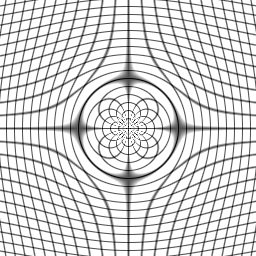
\includegraphics[width=1.0\textwidth]{../images/gridDist.png}
            \caption{Imagem Alvo.}
          \end{center}
        \end{figure}
    \end{columns}
\end{frame}

\begin{frame}
   \begin{columns}[c]
      \column{.5\textwidth}
        A segunda transformação é dada por:
        \begin{align}
        \begin{split}
            X &= x - 8sin(x/32) \\
            Y &= y + 4cos(x/16)
        \end{split} 
        \end{align}
      \column{.5\textwidth}
        \begin{figure}[!h]
          \begin{center}
            
\includegraphics[width=1.0\textwidth]{../images/gridSin.png}
            \caption{Imagem Alvo.}
          \end{center}
        \end{figure}
    \end{columns}
\end{frame}

\begin{frame}
   \begin{columns}[c]
      \column{.5\textwidth}
        A última transformação é dada pela combinação das duas:
        \begin{align}
        \begin{split}
            X &= x - 8sin(x/32) \\
            Y &= y + 4cos(x/16)
        \end{split} 
        \end{align}
      \column{.5\textwidth}
        \begin{figure}[!h]
          \begin{center}
            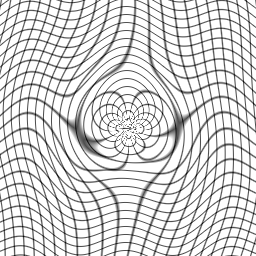
\includegraphics[width=1.0\textwidth]{../images/movingImageDistSin.png}
            \caption{Imagem Alvo.}
          \end{center}
        \end{figure}
    \end{columns}
\end{frame}

\begin{frame}
   \begin{columns}[c]
      \column{.5\textwidth}
        As características do TPS foram gerados usando uma grade uniforme de pontos:
        \begin{figure}[!h]
          \begin{center}
            
\includegraphics[width=1.0\textwidth]{../images/staticCPSSin.png}
            \caption{Imagem Alvo.}
          \end{center}
        \end{figure}
      \column{.5\textwidth}
        Que depois foi deformada pela função em questão:
        \begin{figure}[!h]
          \begin{center}
            
\includegraphics[width=1.0\textwidth]{../images/movingCPSSin.png}
            \caption{Imagem Alvo.}
          \end{center}
        \end{figure}
    \end{columns}
\end{frame}

\section{Resultados}
\subsection{}

\begin{frame}
   \begin{columns}[c]
      \column{.5\textwidth}
        A imagem referência:
        \begin{figure}[!h]
          \begin{center}
            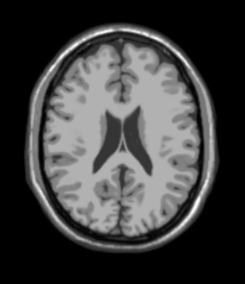
\includegraphics[width=0.9\textwidth]{../images/screen.png}
            \caption{Imagem referência.}
          \end{center}
        \end{figure}
      \column{.5\textwidth}
       A imagem deformada pela função de distância inversa:
        \begin{figure}[!h]
          \begin{center}
            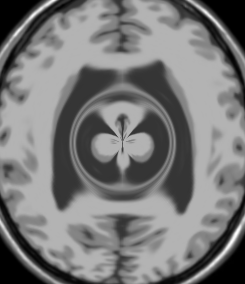
\includegraphics[width=0.9\textwidth]{../images/movingImageDist.png}
            \caption{Imagem Alvo.}
          \end{center}
        \end{figure}
    \end{columns}
\end{frame}

\begin{frame}
   \begin{columns}[c]
      \column{.5\textwidth}
        A imagem deformada pela função senoidal:
        \begin{figure}[!h]
          \begin{center}
            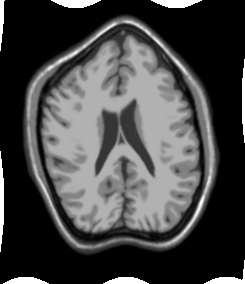
\includegraphics[width=0.9\textwidth]{../images/movingImageSin.png}
            \caption{Imagem referência.}
          \end{center}
        \end{figure}
      \column{.5\textwidth}
       A imagem deformada pela combinação das duas funções:
        \begin{figure}[!h]
          \begin{center}
            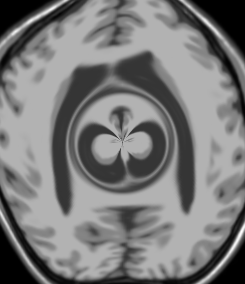
\includegraphics[width=0.9\textwidth]{../images/movingImageSinDist.png}
            \caption{Imagem Alvo.}
          \end{center}
        \end{figure}
    \end{columns}
\end{frame}

\begin{frame}
   \begin{columns}[c]
      \column{.5\textwidth}
        TPS para a senoidal:
        \begin{figure}[!h]
          \begin{center}
            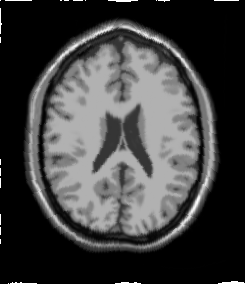
\includegraphics[width=0.9\textwidth]{../images/resultSin.png}
            \caption{Imagem referência.}
          \end{center}
        \end{figure}
      \column{.5\textwidth}
        Demons para a senoidal:
        \begin{figure}[!h]
          \begin{center}
            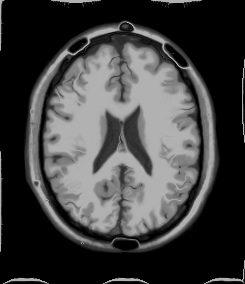
\includegraphics[width=0.9\textwidth]{../images/resultSinDemon.png}
            \caption{Imagem Alvo.}
          \end{center}
        \end{figure}
    \end{columns}
\end{frame}

\begin{frame}
   \begin{columns}[c]
      \column{.5\textwidth}
        TPS para a direção inversa:
        \begin{figure}[!h]
          \begin{center}
            
\includegraphics[width=0.9\textwidth]{../images/resultDist.png}
            \caption{Imagem referência.}
          \end{center}
        \end{figure}
      \column{.5\textwidth}
       Demons para a direção inversa:
        \begin{figure}[!h]
          \begin{center}
            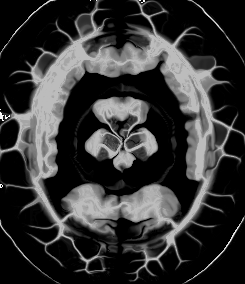
\includegraphics[width=0.9\textwidth]{../images/resultDistDemons.png}
            \caption{Imagem Alvo.}
          \end{center}
        \end{figure}
    \end{columns}
\end{frame}

\begin{frame}
   \begin{columns}[c]
      \column{.5\textwidth}
        TPS para a combinada:
        \begin{figure}[!h]
          \begin{center}
            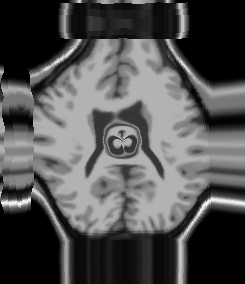
\includegraphics[width=0.9\textwidth]{../images/resultDistSin.png}
            \caption{Imagem referência.}
          \end{center}
        \end{figure}
      \column{.5\textwidth}
       Demons para a combinada:
        \begin{figure}[!h]
          \begin{center}
            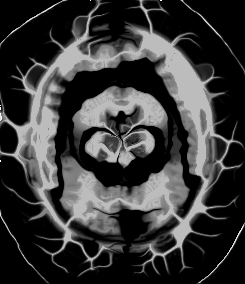
\includegraphics[width=0.9\textwidth]{../images/resultSinDistDemon.png}
            \caption{Imagem Alvo.}
          \end{center}
        \end{figure}
    \end{columns}
\end{frame}

\begin{frame}
    Considerações sobre o Demons:
    \begin{itemize}
        \item Como o Demons utiliza o gradiente das duas imagens para definir a direção dos vetores, ele é sensível a deformações bruscas, como a distância inversa;
        \item O Demons utiliza um filtro gaussiano a cada iteração, introduzindo uma suavização a imagem.
    \end{itemize}
\end{frame}

\begin{frame}
    Considerações sobre o TPS:
    \begin{itemize}
        \item Como os pontos de controles foram gerados de maneira uniforme, as transformações jogaram alguns pontos para fora da imagem prejudicando a sua eficácia;
        \item Ele obtém melhores resultados porém não é tão rápido quanto o Demons.
    \end{itemize}
\end{frame}

\section{Conclusão}
\subsection{}

\begin{frame}
    O TPS gerou os melhores resultados no geral. \\
    O Demons obtêm resultados aceitáveis dado que a transformação seja uniforme. \\
    Um próximo passo para o estudo é a aceleração do TPS e a utilização de um algoritmo para a determinação das características.
\end{frame}

\section{Bibliografia}
\subsection{}

\begin{frame}[allowframebreaks]
  \frametitle{Referências}    
  \framesubtitle{}
  \bibliographystyle{amsalpha}
  \bibliography{bibliografia}{}
\end{frame}
\end{document}